% Created 2020-12-31 Thu 14:24
% Intended LaTeX compiler: pdflatex
\documentclass[a4paper]{report}
\usepackage[utf8]{inputenc}
\usepackage[T1]{fontenc}
\usepackage{graphicx}
\usepackage{grffile}
\usepackage{longtable}
\usepackage{wrapfig}
\usepackage{rotating}
\usepackage[normalem]{ulem}
\usepackage{amsmath}
\usepackage{textcomp}
\usepackage{amssymb}
\usepackage{capt-of}
\usepackage{hyperref}
\usepackage[francais, english]{babel}
\usepackage{graphicx}
\date{\today}
\title{}
\hypersetup{
 pdfauthor={},
 pdftitle={},
 pdfkeywords={},
 pdfsubject={},
 pdfcreator={Emacs 27.1 (Org mode 9.3)}, 
 pdflang={English}}
\begin{document}

\begin{LaTex}
\begin{titlepage}
\centering
  {\scshape Hénallux\par\vspace{0.2cm} Section sécurité des systèmes\par \vspace{0.2cm}}
  \vspace{1cm}
  
\includegraphics[width=0.5\textwidth]{img/school}\par\vspace{1cm}
  {\scshape \LARGE Développement \par}
  \vspace{0.2cm}
	{\scshape \Large Implémentation d'un IDS\par}
  \vspace{3cm}
  {\Large\itshape Projet réalisé par \par\vspace{0.5cm} Mustafa-Can KUS \par Jordan DALCQ \par}
  \vfill
  \scshape Année académique 2020-2021 
  \title{Implémentation d'un IDS}
  \author{Mustafa-Can KUS Jordan DALCQ}
  \date{2020-2021}
\end{titlepage}

\pagestyle{headings}
\end{LaTex}
\tableofcontents

\part{Introduction}
\label{sec:org7800537}
\chapter{Contexte}
\label{sec:orgb0ec95b}
Dans le cadre du cours de développement il nous a été demandé de réalisé un système de détection d'intrusion (ou IDS pour faire plus cours).
Ce programme à pour but d'analyser le trafique réseau et reporter toutes activité suspectes à un administrateur système ou même un administrateur réseau
grâce à un système de log.

\chapter{Outils utilisés}
\label{sec:org8e3225b}
\section{Org mode}
\label{sec:org0e1ee43}
Org mode est un mode majeur pour le logiciel GNU Emacs qui permet de prendre notes et maintenir une Todo liste et permet aussi de planifier facilement des projets
grâce à son langage Markup (très proche du markdown). On l'a utilisé pour écrire ce report (ok on a un peu tricher on a mit un peu de Latex pour faire joli) et aussi
pour planifier notre travail 

\begin{figure}[htbp]
\centering
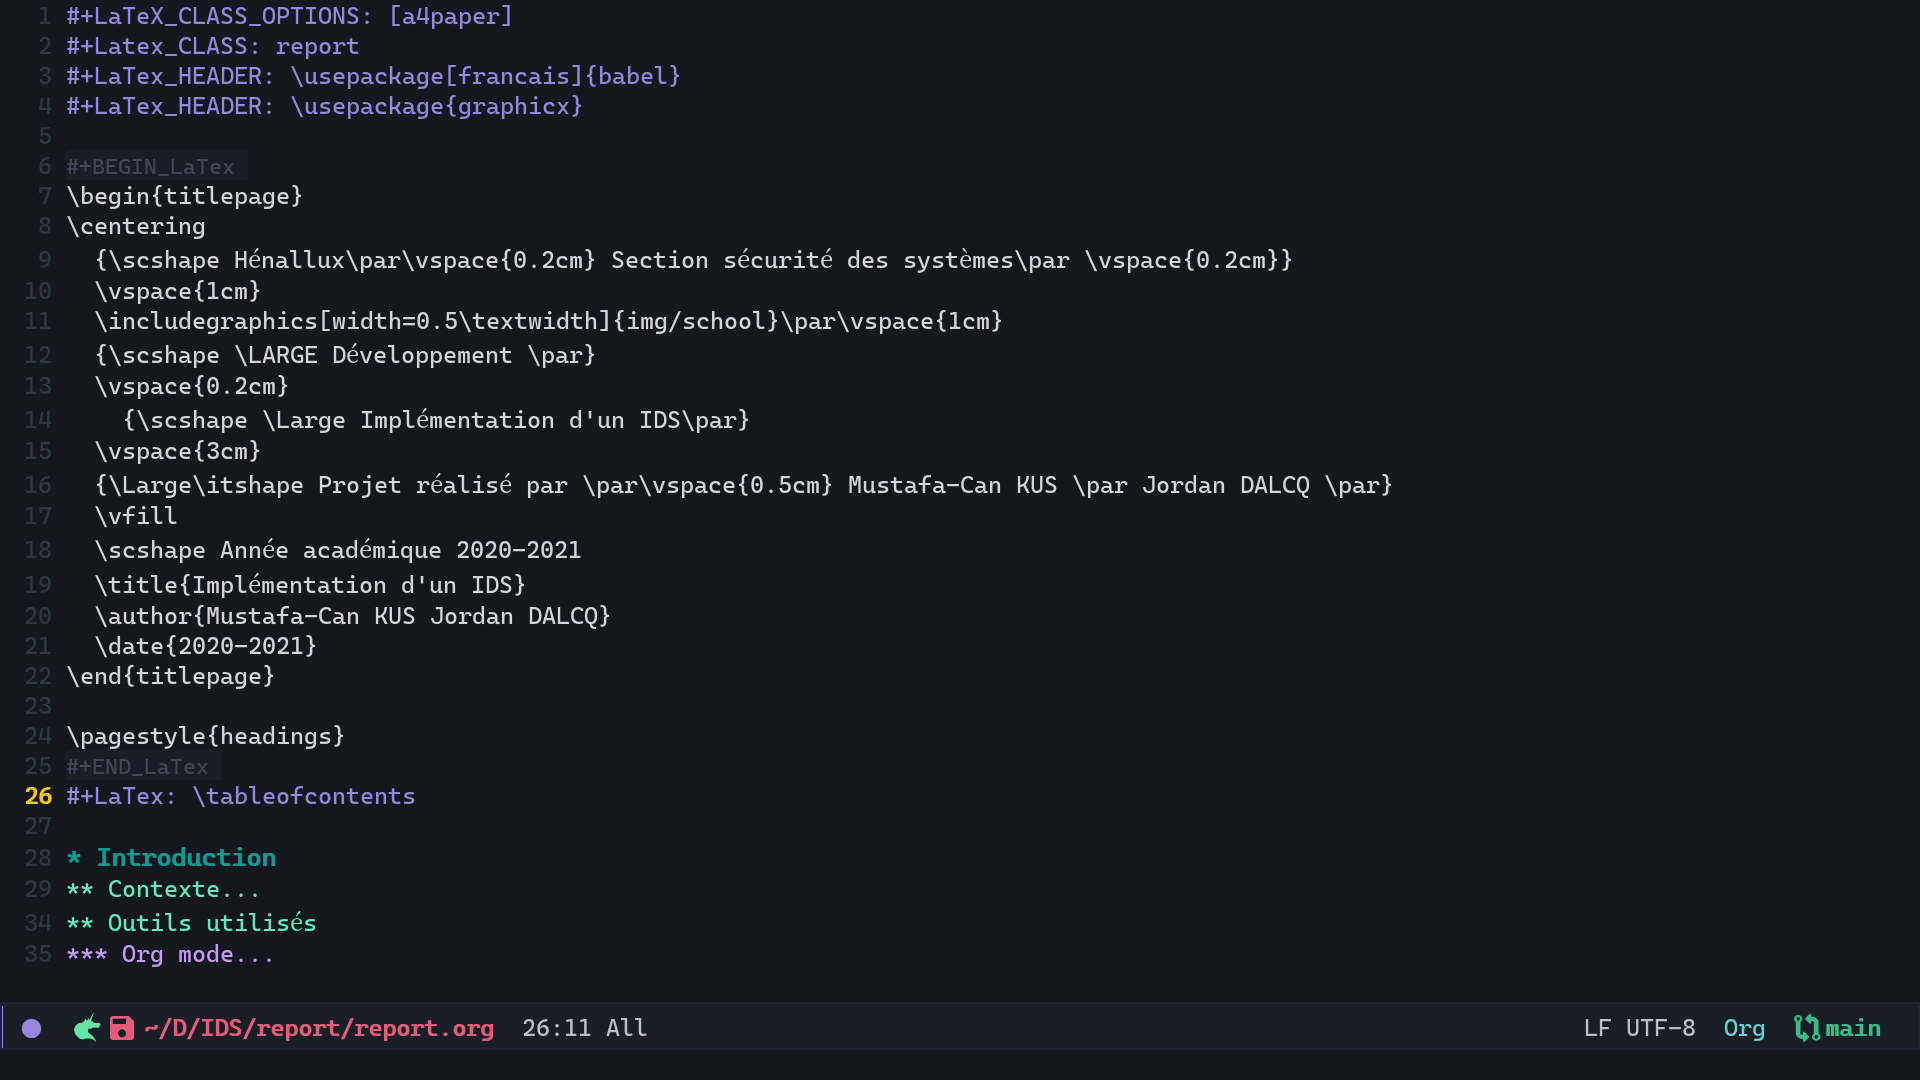
\includegraphics[width=.9\linewidth]{./img/org.png}
\caption{\label{fig:org498c5f6}Capture d'écran de notre rapport écrit avec l'Org mode}
\end{figure}
\section{Github}
\label{sec:orga820e72}
Une fois notre planing fait il nous fallait une solution pour que chaqu'un d'entre nous aie une copie du code toujours à jours 
et qu'on puisse tracker nos modifications, ce qui est très pratique en cas de bug, en effet il nous aurait suffit que de revenir 
quelques modifications en arrière et le problème est régler !

Notre projet est disponible ici:
\begin{LaTex}
\begin{center}
    {\small \url{https://github.com/Les-IRaniens/IDS}}
\end{center}
\end{LaTex}
\section{GNU Makefile}
\label{sec:orgd4f8571}
Comme tous bon informaticiens qui se respecte, on a pas envie de tapper une très longue commande composé d'une dixène de fichiers et d'une
autres dixène de flag à chaque fois qu'on souhaite compiler notre programme, alors on a décider d'utiliser un makefile. 
Le makefile s'occupe de compiler et de linker notre code automatiquement, il suffit de tapper make dans le terminal et le tour est jouer !
\section{Nos flags de compilations}
\label{sec:orgacd67b3}
\begin{itemize}
\item -pednatic: nous oblige fortement à adhérer aux règles de l'ANSI C
\item -Wpednatic: nous affiche des warnings si on respecte pas la pedantic
\item -Wall: nous permet d'avoir tous les warnings sur des pratiques considérées comme questionnable
\item -Wextra: Couvre encore plus de warnings que -Wall
\item -Werror: Transforme tous les warnings en erreur (Oui on est sans pitier ici)
\item -g: Permet d'avoir les symboles de debugger
\item -Isrc/: Permet d'inclure facilement les headers du dossier src
\item -fsanitize=undefined \& -fsanitize=undefined: Permet de tracker chaque memory leaks et nous dit sur quelle ligne est le problème
\item -lpcap: Inclus la libpcap à notre projet
\end{itemize}

\section{ArchLinux}
\label{sec:orgcff1eca}
Programmer sur Kali c'est pas top, surtout sur une VM ! Donc on a préférer utiliser ArchLinux pour le travail sur machine native.
Pourquoi celà ? Car Archlinux est une distribution polyvalante qui a TOUS les paquets qu'on désire (oui même tous les paquets de Kali)
\section{Vscodium}
\label{sec:orga96acb4}
C'est Visual Studio Code - les fonctions de télémétries, c'est notre éditeur de choix, car il permet une super bonne intégration avec notre github,
nous informe de nos erreurs et des warnings potentiels grâce à l'extension C/C++.
\end{document}
